\section{Electronic market making}
    We need to define the market making problem in the market. As it was stated in \cite{Cartea2015} and \cite{Bouchaud2018},
    the objective of the electronic market is to match the buy and sell orders 
    of the market participants. In practice we can divide all orders to 
    the two groups: \emph{market orders} (MO) and \emph{limit orders} (LO). 
    \begin{definition}
        A \emph{limit order} is an order to buy or sell a security at a specific price or better. This type of order guarantees the execution price, but does not guarantee the execution itself.
    \end{definition}
    \begin{definition}
        A \emph{market order} is an order to buy or sell a security immediately. This type of order guarantees that the order will be executed, but does not guarantee the execution price.
    \end{definition}
    
    The limit orders are \emph{passive}, i.e. they are not executed immediately, since 
    we need to find a counterparty for them. The market orders are \emph{aggressive},
    i.e. they are executed immediately, since they are the ones being dynamically matched with the limit orders. 
    The market orders for $N$ shares collects the best $N$ shares limit orders from the order book.
    The order book stores only the information about the limit orders, so we can call it the limit order book (LOB).
    If the market order is larger than the best priced limit order, then the remaining part of the 
    market order is executed via the second best limit order from the LOB. Because of that, the current 
    market price of the asset moves in the direction of the market order.

    This effect is called a \emph{price impact} and it is the main reason why we should need to 
    optimize the trade execution. The price impact could be represented as a function of the order size and the time.
    If we execute the MO rapidly, then we will pay a lot of money for the price impact. We should 
    note that the price impact has the inverse relation with the liquidity of the asset. The more liquid the asset is, the less price impact is.
    If we execute only the best priced limit orders in order to avoid the price impact of the certain assets, then we are 
    doomed to be executing the MO for quite a long time, what significantly increases the \emph{market risk}. The market 
    risk is the risk of the drastic price change during the execution horizon. Therefore, we found a trade-off between the 
    price impact and the market risk.
    
    Now we are ready to formulate the \emph{optimal execution problem}: liquidate the position by minimizing the functional of the price impact and the market risk. 
    Let us write this problem in terms of stochastic optimal control.

    Let us have $X$ lots of an asset in the long position that we need to sell during time $T$ from now.
    Let us have $N$ stock exchange ticks and we define the \emph{liquidation times} $t_k = k\tau$, $\tau = T/N$.
    \begin{definition}
        The \emph{trading trajectory} is a process $(x_k)_{k = 0, \dots, N}$, where $x_k$ is a number of lots we 
        still posess at time $t_k$. Alternatively, we can define the \emph{trade list} $n_k = \Delta x_k$, $k = 1, \dots, N$ as a 
        number of lots we sell at time $t_k$.
        The \emph{trading strategy} is a rule for determining $n_k$ given the information avaliable at time $t_k$. Mathematically speaking,
        \begin{equation*}
            \hat n_k = \mathbb{E}^\nu\left[n_k\vert \mathcal{F}_{t_{k-1}}\right]. 
        \end{equation*} 
    \end{definition}
    We can divide the strategies to \emph{static} (deterministic, all the parameters are known upon the start of the execution) and \emph{dynamic} (stochastic).
    Static strategies do not require any learning, but for the dynamic strategies it is often useful to use online machine learning (RL in particular).
    As it was stated in \cite{Cartea2015}, we can differentiate all dynamic traders (same as their correspoding strategies) into the three main classes:
    \begin{enumerate}
        \item \emph{Fundamental traders} (also \emph{noise \emph{or} liquidity traders}): those traders, who exploit some general exogenous economic factors. There is a subtle difference between all three: \begin{itemize}
            \item Fundamental traders usually have some kind of medium or long term strategy,
            \item Noise traders are those who trade orthogonally to the market events, i.e. their actions weakly depend on others,
            \item Liquidity traders are those, who are forced (by their strategy) to exploit the market orthogonally to major events;
        \end{itemize}
        \item \emph{Informed traders}: those traders, who profit from some insider knowledge, a.k.a. information, which is not reflected in the prices;
        \item \emph{Market makers}: professional traders, who have a market power;
        \item Sometimes, the \emph{arbitrageurs} are differentiated as a fourth group. However, they might be considered to be a subclass of the informed traders.
    \end{enumerate}

    \begin{definition}
        The \emph{capture} of the trajectory is the total nominal trading revenue upon completion of the execution:
        \begin{equation*}
            CP(n, S) = \sum_{k=1}^{N} n_kS_k.
        \end{equation*}
        The \emph{total cost} of the trading trajectory is the difference between the capture and the initial book value:
        \begin{equation*}
            TC = XS_0 - CP(n, S).
        \end{equation*}
    \end{definition}
    We define the regret functional for one tick the following way:
    \begin{equation*}
        L(m) = E(m) + \lambda V(m),
    \end{equation*}
    where $m$ is the total price of the position to be liquidated immediately, $E(m)$ is the expected total costs (or \emph{implementation shortfall}, according to the terminology introduced in \cite{Perold1988}), $V(m)$ is the variance of the shortfall, and $\lambda$ is the relative risk propensity:
    \begin{equation*}
        \lambda(w) = -\frac{u''(w)}{u'(w)},
    \end{equation*}
    where $u$ is the utility function of the trader. If our initial portfolio is fully owned, then as we transfer our assets from the risky stock into the alternative investment,
    total wealth remains roughly constant, and we may take $\lambda$ to be constant throughout our trading period.
    
    As it was stated in \cite{Almgren2000}, we must care about the risk when deciding whether we should hold the position. Therefore, $\lambda \ne 0$. Because of that, 
    the utility function is either strictly concave (in case of the risk-averse trader) or strictly convex (in case of the risk-tolerant trader).

\section{Online machine learning and reinforcement learning}
    Online machine learning, also known as incremental or sequential learning, is a type of machine learning where models are learned and improved over time as new data becomes available. Rather than training a model on a fixed dataset all at once, online machine learning allows the model to adapt and evolve in response to changing conditions.

    One of the main benefits of online machine learning is that it can reduce the amount of time and computational resources required for training and updating a model. Rather than starting from scratch each time new data is added, the model can build on previous knowledge, leading to more efficient learning.


\section{Algorithm prerequisites}
    \subsection{Description of the model}
        First of all, we can neglect the time value of money since we are working in the high-frequency
        trading world, i.e. the money do not lose any value in our scale. Therefore, $\gamma \equiv 1$.

        Our trading bot has the following set of actions:
        \begin{itemize}
            \item Hold;
            \item Sell 1 lot of the asset;
            \item Sell 2 lots of the asset;
            \item Sell 3 lots of the asset;
            \item Sell 4 lots of the asset;
            \item etc.
        \end{itemize}
        The number of possible actions depends on the leftover size of the position to be liquidated.
        The bandit stops when there is no other action but to hold the position with 0 assets. 
        The cumulative regret function is the accumulated price impact costs with the correction for the excessive risk.
        It is obvious that the target functional without the risk correction has its $\epsilon$-optimal 
        solution with the uniform distribution of the trades over the given liquidation horizon.
        Therefore, we shall use the TWAP (Time-Weighted Average Price) execution algorithm as a baseline model.
        According to \cite{TWAP}, 
        \begin{quote}
            TWAP trading algorithms seek to optimize a trade's average price while executing over a specified time period. This is generally used to execute large orders that are expected to have significant market impact.
        \end{quote}
        We define the pseudo-regret functional as the accumulated price impact weighted by volume with risk correction:
        \begin{equation}
            \operatorname*{PRegret} = \sum_{k=1}^{T}\hat{n}_k\operatorname*{PriceImpact}(k) + \lambda \rho(n),
        \end{equation}
        where $\rho(n) = \rho(n_1, \dots, n_T)$ is an arbitrary coherent risk measure, $\lambda$ is the relative risk propensity, and $\hat n$ is the realised trading list.

    \subsection{Data collection}
        We obtained the L3 quote data for the four currency pairs from the MOEX:
        \begin{enumerate}
            \item USD/RUB; 
            \item EUR/RUB; 
            \item CHN/RUB;
            \item EUR/USD.
        \end{enumerate} 
        The data is stored in the JSON format and contains the following fields: \inputminted{json}{codeminted/l3quote.json}
        \noindent The estimated size of the data is about 80 Gb. 
        
    \subsection{Order book implementation}
        We implemented the order book in Rust using the B-tree as a base data structure (See \Cite{Cormen2022}). To our knowledge, 
        the ring buffer is considered to be the best practice in the industrial tasks for the order book storing, but we used 
        the B-tree due to the ease of the implementation.
        In order to effectively search the order book, we implemented the hash map contating the IDs of the quotes and
        the price levels at which the order is placed. The \mintinline{rust}|OrderBook| struct contains the following fields:
        \begin{enumerate}
            \item \mintinline{rust}|instrument|: a field containing the name of the asset;
            \item \mintinline{rust}|bid| and \mintinline{rust}|ask|: sides of an order book. They are 
                  stored as a B-tree with price levels as keys and queues of L3 quotes as the items correspoding
                  to the price levels.
            \item \mintinline{rust}|price_step| and \mintinline{rust}|price_step_inv| are needed to calculate the 
                  price level of the correspoding order. \mintinline{rust}|key = price*price_step_inv|.
        \end{enumerate}
        The data is read from the raw MOEX files using the \href{https://github.com/serde-rs/json}{\texttt{serde-rs/json}} library. Then, the obtained data is
        converted into the \mintinline{rust}|OrderBook| structure tick-by-tick using the \mintinline{rust}|OrderBook::update()| method.

    \subsection{Features calculation}
        To calibrate the trading bandit, we calculated the following parameters from the LOB:
        \begin{itemize}
            \item price-by-volume $P(Q)$;
            \item volume-by-price-threshold $Q(dP)$, $dP$ is the maximal possible price impact;
            \item Imbalance of the previous parameters\begin{itemize}
                \item $I_1(Q) = (\texttt{Ask}(Q) - \texttt{Ask}(0)) - (\texttt{Bid}(0) - \texttt{Bid}(Q))$,
                \item $I_2(dP) = Q(\texttt{Ask} - \texttt{BestAsk}) - Q(\texttt{Bid} - \texttt{BestBid})$.
            \end{itemize}
        \end{itemize}

\section{Online learning algorithm for optimal execution in the limit order book}
    \begin{definition}
        \emph{Average Cost Per Round} (ACPR)
        \begin{align}
            & \operatorname*{ACPR} = \frac{1}{\operatorname{num\_of\_rounds}} \sum_\rho IS_\rho,\\
            & IS_\rho = (W \operatorname{mid}(\rho, 1) - \sum_l A^\rho_l \operatorname{bid}(\rho, l))/(W\operatorname{mid}(\rho, 1)).
        \end{align}
    \end{definition}
    \subsection{TWAP}
        The simplest execution algorithm.
        \begin{figure}
            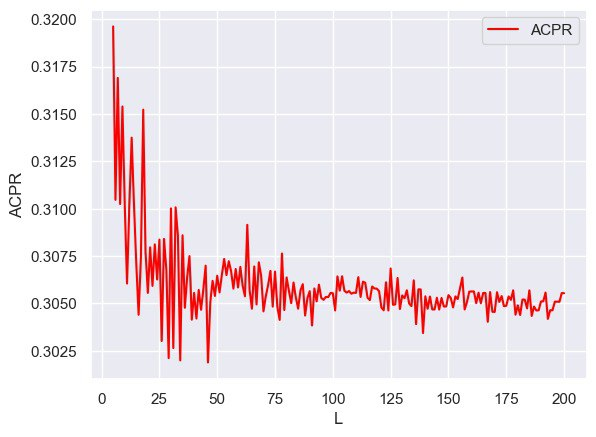
\includegraphics[width=0.9\textwidth]{twap_acpr.png}
            \caption{TWAP ACPR dynamics. $T = 200$.}
        \end{figure}

    \subsection{AC}

    \subsection{GLOBE}
        The following algorithm was introduced in \cite{Akbarzadeh2018}.
        \begin{algorithm}
            \caption[GLOBE Algorithm]{Greedy exploitation in Limit Order Book Execution (GLOBE)}
            \begin{algorithmic}
                \State Input: $L, \mathcal{M}, \mathcal{M}^r$
                \State Initialize: $\rho = 1, N(M)=0, N(M,M)=0, \forall M \in \mathcal{M}^r , \forall M' \in \mathcal{M}$
                \While {$\rho < 1$}
                    \State $\hat P_\rho (M, M') := \frac{N(M, M') + \1(N(M) = 0)}{N(M) + |\mathcal M| \1 (N(M) = 0)}$
                    \State Update $\sigma_\rho$ in the AC model based on the past observations
                    \State Observe $X_\rho = (W_\rho, p_r(\rho), \sigma_\rho, B_1^\rho)$
                    \State Compute $A_l$ based on the AC model $\forall l \in \mathcal{L}$
                    \State Compute the estimated optimal policy by dynamic programming using the action set $\mathcal A_l^*$, $\forall l \in \mathcal{L} - \{L\}$ and $\hat P_\rho (M, M') \forall M \in \mathcal{M}^r, \forall M' \in \mathcal M$
                    \State $I_1^\rho = W_\rho$, $l=1$
                    \While {$l < L$}
                        \State Observe $M_l^\rho$, sell $a_l^\rho\in \mathcal{A}^*_l$ using the estimated policy
                        \State Calculate $C_{X_\rho}(M_l^\rho, a_l^\rho)$
                        \State $I_{l+1}^\rho = I_l^\rho - a_l^\rho$
                        \State $l\ +\!\!=1$
                    \EndWhile
                    \State $a_{L}^\rho := I_L^\rho$
                    \State $\rho\ +\!\!= 1$
                    \State Update $N(M, M')$ and $N(M)$ $\forall M \in \mathcal{M}^r$ according to \eqref{globe:rule1} and \eqref{globe:rule2}
                \EndWhile
            \end{algorithmic}
        \end{algorithm}
        \begin{align}
            & N \label{globe:rule1}\\
            & N \nonumber\\
            & P \label{globe:rule2}
        \end{align}